
This chapter presents the experimental results obtained from the EpiDetect pipeline. All experiments were conducted on the Bonn University EEG dataset using 10-fold stratified cross-validation with multi-seed ensemble training.

\section{Experimental Setup}

\subsection{Dataset}

The Bonn University EEG dataset~\citep{andrzejak2001indications} consists of 500 single-channel EEG recordings, each containing 4097 amplitude values sampled at 173.61~Hz (approximately 23.6 seconds per recording). The data is organized into five clinical sets:

\begin{table}[htbp]
\centering
\renewcommand{\arraystretch}{1.3}
\caption{Bonn University EEG Dataset Composition.}
\label{tab:dataset}
\begin{tabular}{|c|c|l|c|c|}
\hline
\textbf{Set} & \textbf{Letter} & \textbf{Subject / State} & \textbf{Signals} & \textbf{Label} \\
\hline
A & Z & Healthy volunteer, eyes open & 100 & 0 (Normal) \\
\hline
B & O & Healthy volunteer, eyes closed & 100 & 0 (Normal) \\
\hline
C & N & Epileptic patient, seizure-free zone & 100 & 0 (Normal) \\
\hline
D & F & Epileptic patient, epileptogenic zone & 100 & 0 (Normal) \\
\hline
E & S & Epileptic patient, during seizure & 100 & 1 (Seizure) \\
\hline
\multicolumn{3}{|r|}{\textbf{Total}} & \textbf{500} & \\
\hline
\end{tabular}
\end{table}

The binary classification task groups Sets A--D as the non-seizure class (400 signals) and Set E as the seizure class (100 signals), producing a 4:1 class imbalance. This imbalance is addressed through class weighting (seizure weight = 4.0) in classifiers that support it.

Figure~\ref{fig:eegsignals} shows a representative EEG signal from each of the five sets. The healthy signals (Sets Z and O) exhibit relatively regular, low-amplitude oscillations. The inter-ictal recordings (Sets N and F), captured from epileptic patients between seizures, show slightly elevated irregularity. Set S (seizure) displays the characteristic high-amplitude, chaotic spikes that distinguish ictal activity from all other brain states.

\begin{figure}[htbp]
\centering
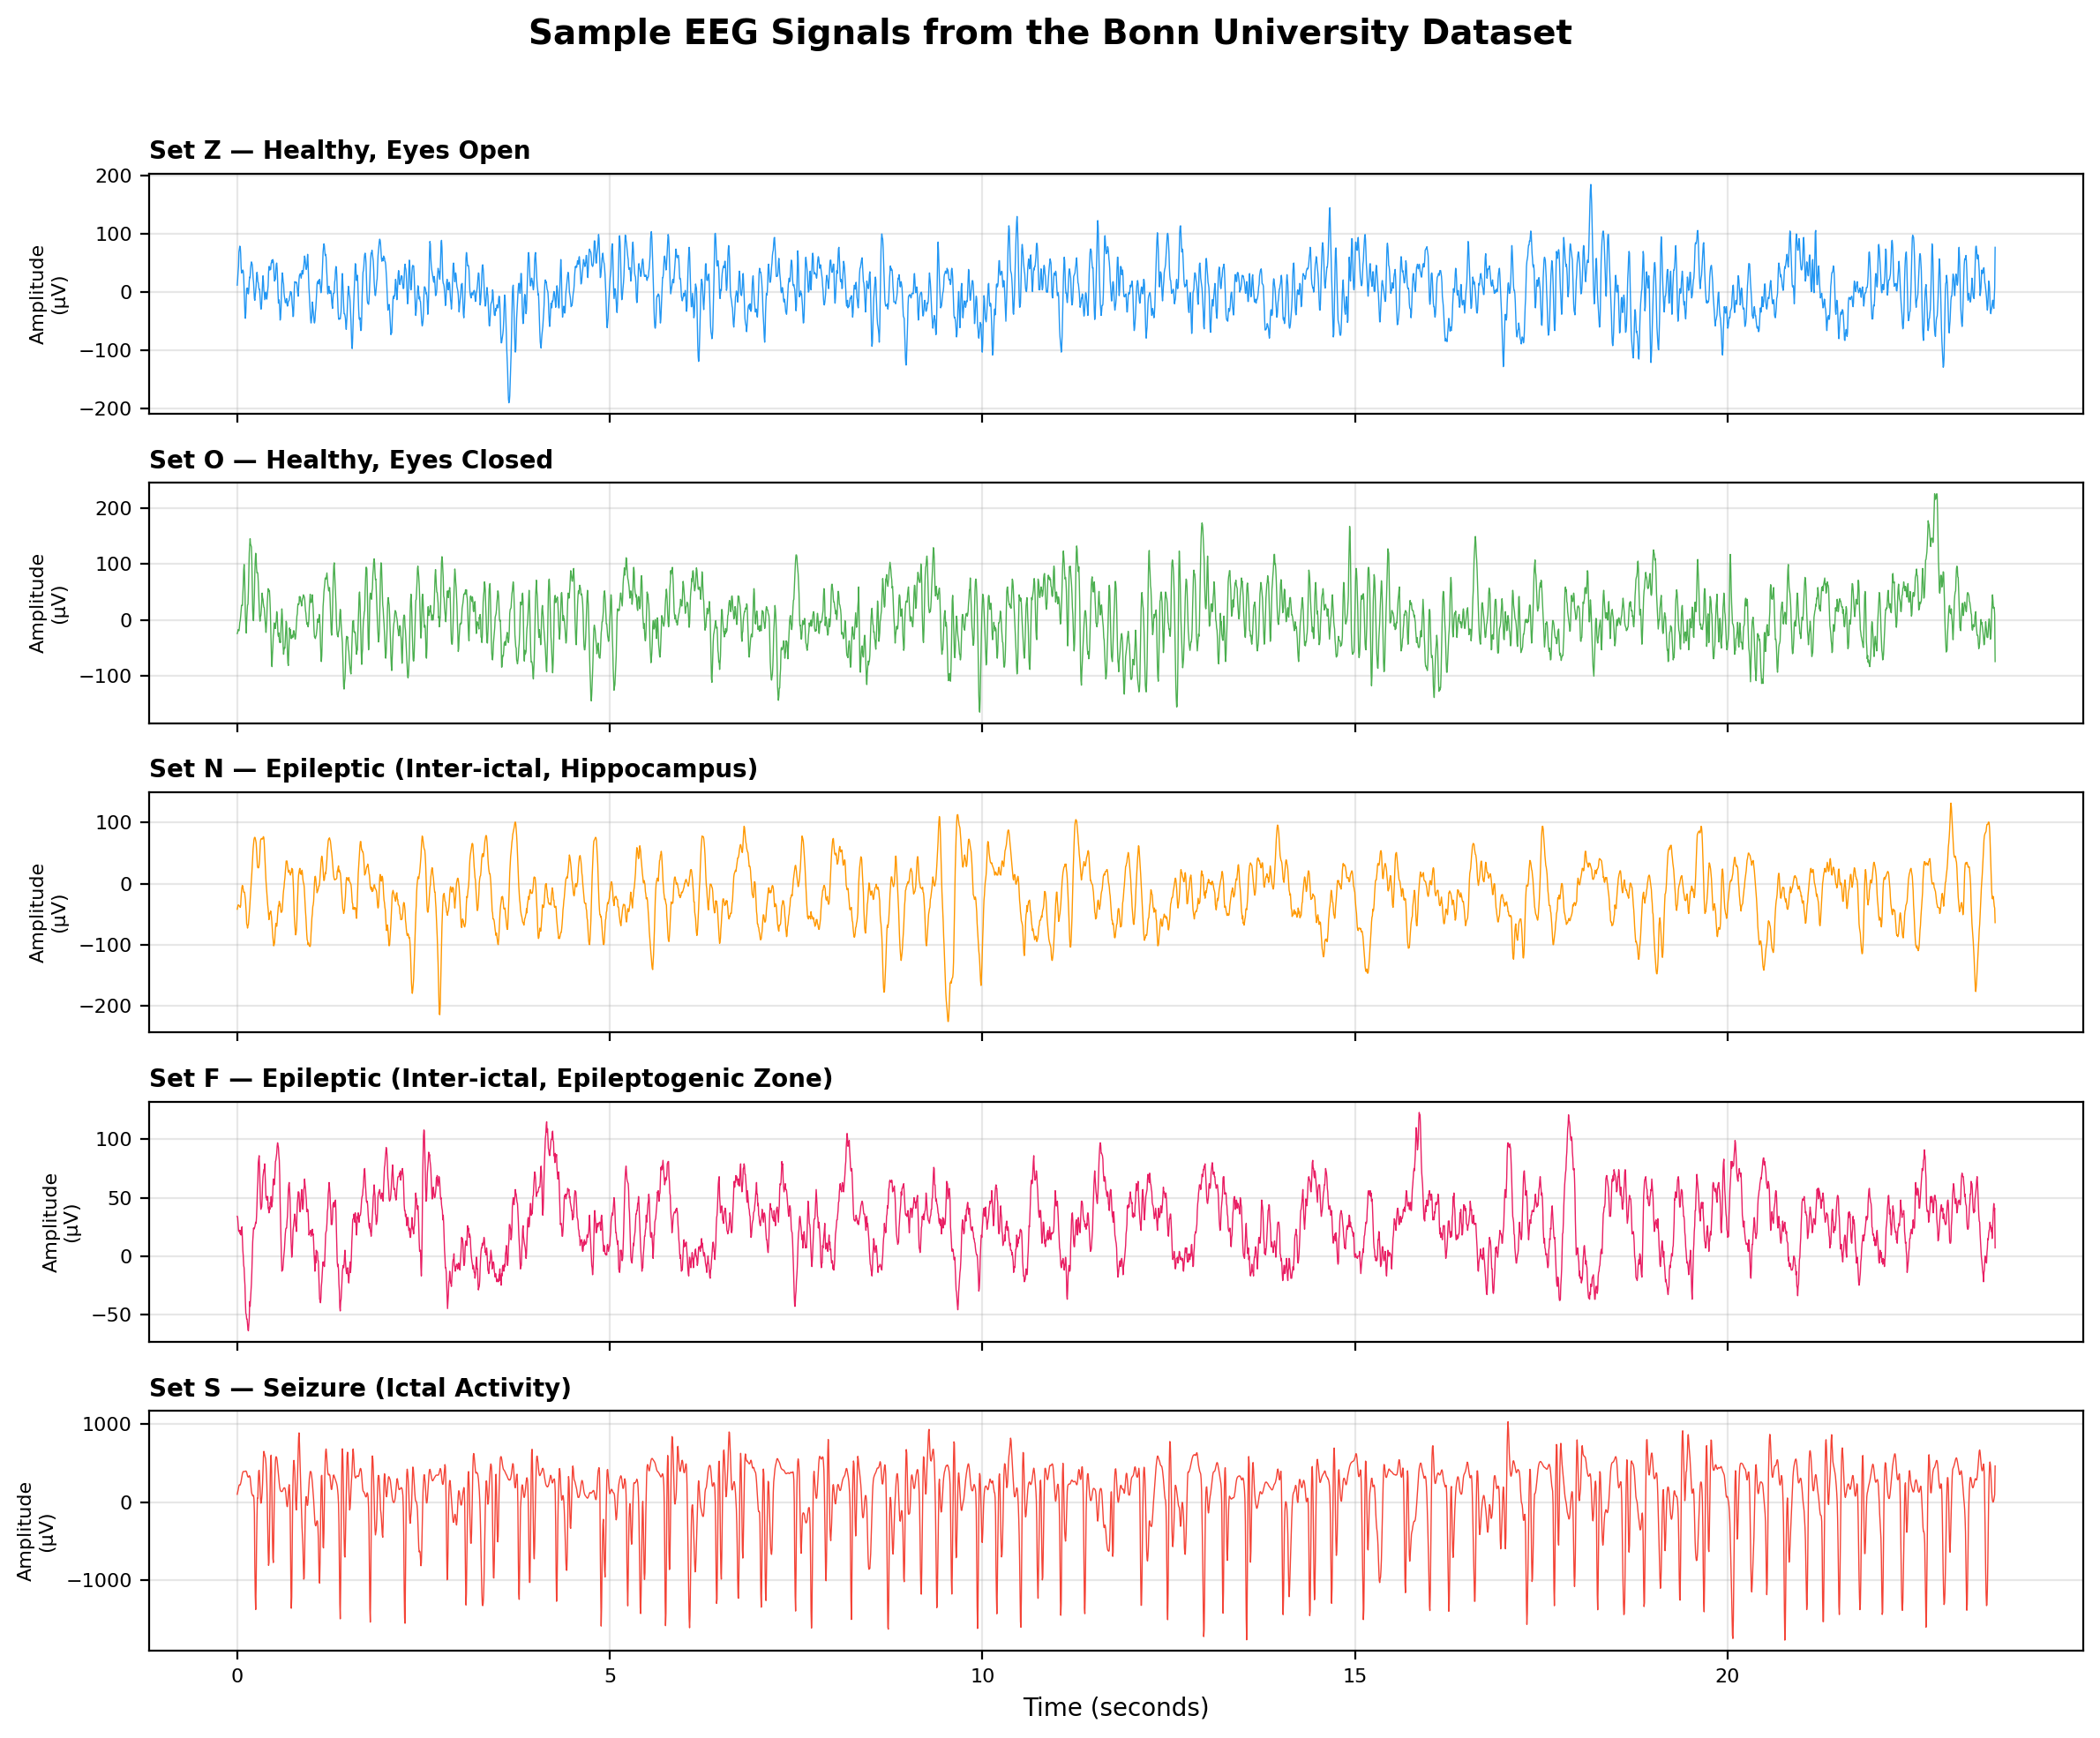
\includegraphics[width=\textwidth]{images/eeg_signals.png}
\caption{Sample EEG waveforms from each set of the Bonn University dataset.}
\label{fig:eegsignals}
\end{figure}

\subsection{Evaluation Protocol}

All results are reported under 10-fold stratified cross-validation. Stratification ensures that each fold preserves the 4:1 class ratio. Within each fold, the training data is used to fit the scaler, feature selectors, and classifiers, while the test data remains unseen until evaluation. Seven metrics are computed per fold: accuracy, precision, recall, F1-score, AUC-ROC, specificity, and Cohen's kappa.

\subsection{Training Configuration}

Key hyperparameters used in the experiments are listed below:

\begin{table}[htbp]
\centering
\renewcommand{\arraystretch}{1.25}
\caption{Training Hyperparameters.}
\label{tab:hyperparams}
\begin{tabular}{|l|l|}
\hline
\textbf{Parameter} & \textbf{Value} \\
\hline
Cross-validation folds & 10 (stratified) \\
\hline
Random seeds & \{42, 123, 456, 789, 2024\} \\
\hline
Feature selection (per method) & Top 200 \\
\hline
Classification threshold & 0.5 \\
\hline
Seizure class weight & 4.0 \\
\hline
RF / ET estimators & 500 trees \\
\hline
HGB iterations & 400 \\
\hline
GBM estimators & 300 \\
\hline
AdaBoost estimators & 200 \\
\hline
MLP architecture & (256, 128, 64) with early stopping \\
\hline
SVM kernel / C & RBF / 20.0 \\
\hline
KNN neighbours & 5 (distance weighted) \\
\hline
\end{tabular}
\end{table}

\section{Overall Classification Results}

Table~\ref{tab:overall} presents the mean and standard deviation of each metric across 10 folds.

\begin{table}[htbp]
\centering
\renewcommand{\arraystretch}{1.4}
\caption{Overall Classification Performance (10-Fold CV).}
\label{tab:overall}
\begin{tabular}{|l|c|}
\hline
\textbf{Metric} & \textbf{Mean $\pm$ Std (\%)} \\
\hline
Accuracy & 99.40 $\pm$ 0.92 \\
\hline
Precision & 99.09 $\pm$ 2.73 \\
\hline
Recall (Sensitivity) & 98.00 $\pm$ 4.00 \\
\hline
F1-Score & 98.47 $\pm$ 2.34 \\
\hline
AUC-ROC & 99.92 $\pm$ 0.23 \\
\hline
Specificity & 99.75 $\pm$ 0.75 \\
\hline
Cohen's Kappa & 98.10 $\pm$ 2.91 \\
\hline
\end{tabular}
\end{table}

The results show that the system achieves near-perfect classification on the Bonn dataset. The accuracy of 99.40\% means that out of 500 signals, only 3 were misclassified across all folds. The AUC-ROC of 99.92\% indicates excellent discrimination between the two classes across all probability thresholds.

The relatively higher standard deviation in recall (4.00\%) is expected given the class imbalance: with only 10 seizure signals per fold, a single misclassification has a larger proportional impact on seizure-class recall than on overall accuracy.

\section{Confusion Matrix}

Table~\ref{tab:confusion} presents the aggregated confusion matrix across all 10 folds.

\begin{table}[htbp]
\centering
\renewcommand{\arraystretch}{1.4}
\caption{Aggregated Confusion Matrix (All Folds Combined).}
\label{tab:confusion}
\begin{tabular}{|l|c|c|}
\hline
 & \textbf{Predicted Normal} & \textbf{Predicted Seizure} \\
\hline
\textbf{Actual Normal} & 399 & 1 \\
\hline
\textbf{Actual Seizure} & 2 & 98 \\
\hline
\end{tabular}
\end{table}

Out of 500 signals:
\begin{itemize}
    \item \textbf{True Negatives (399):} Normal signals correctly classified as normal.
    \item \textbf{True Positives (98):} Seizure signals correctly detected.
    \item \textbf{False Positives (1):} One normal signal incorrectly flagged as seizure.
    \item \textbf{False Negatives (2):} Two seizure signals missed by the classifier.
\end{itemize}

The total error count of 3 out of 500 confirms the high reliability of the ensemble approach. Figure~\ref{fig:metrics_bar} presents a bar chart visualization of these classification metrics. The bar chart is significant because it makes the asymmetry across metrics immediately visible: specificity, AUC-ROC, and accuracy all sit above 99\%, while recall (sensitivity) sits slightly lower at 98\%, reflecting that the two missed seizure signals impact the seizure-class recall more than they affect the overall accuracy on the imbalanced dataset.

\begin{figure}[htbp]
\centering
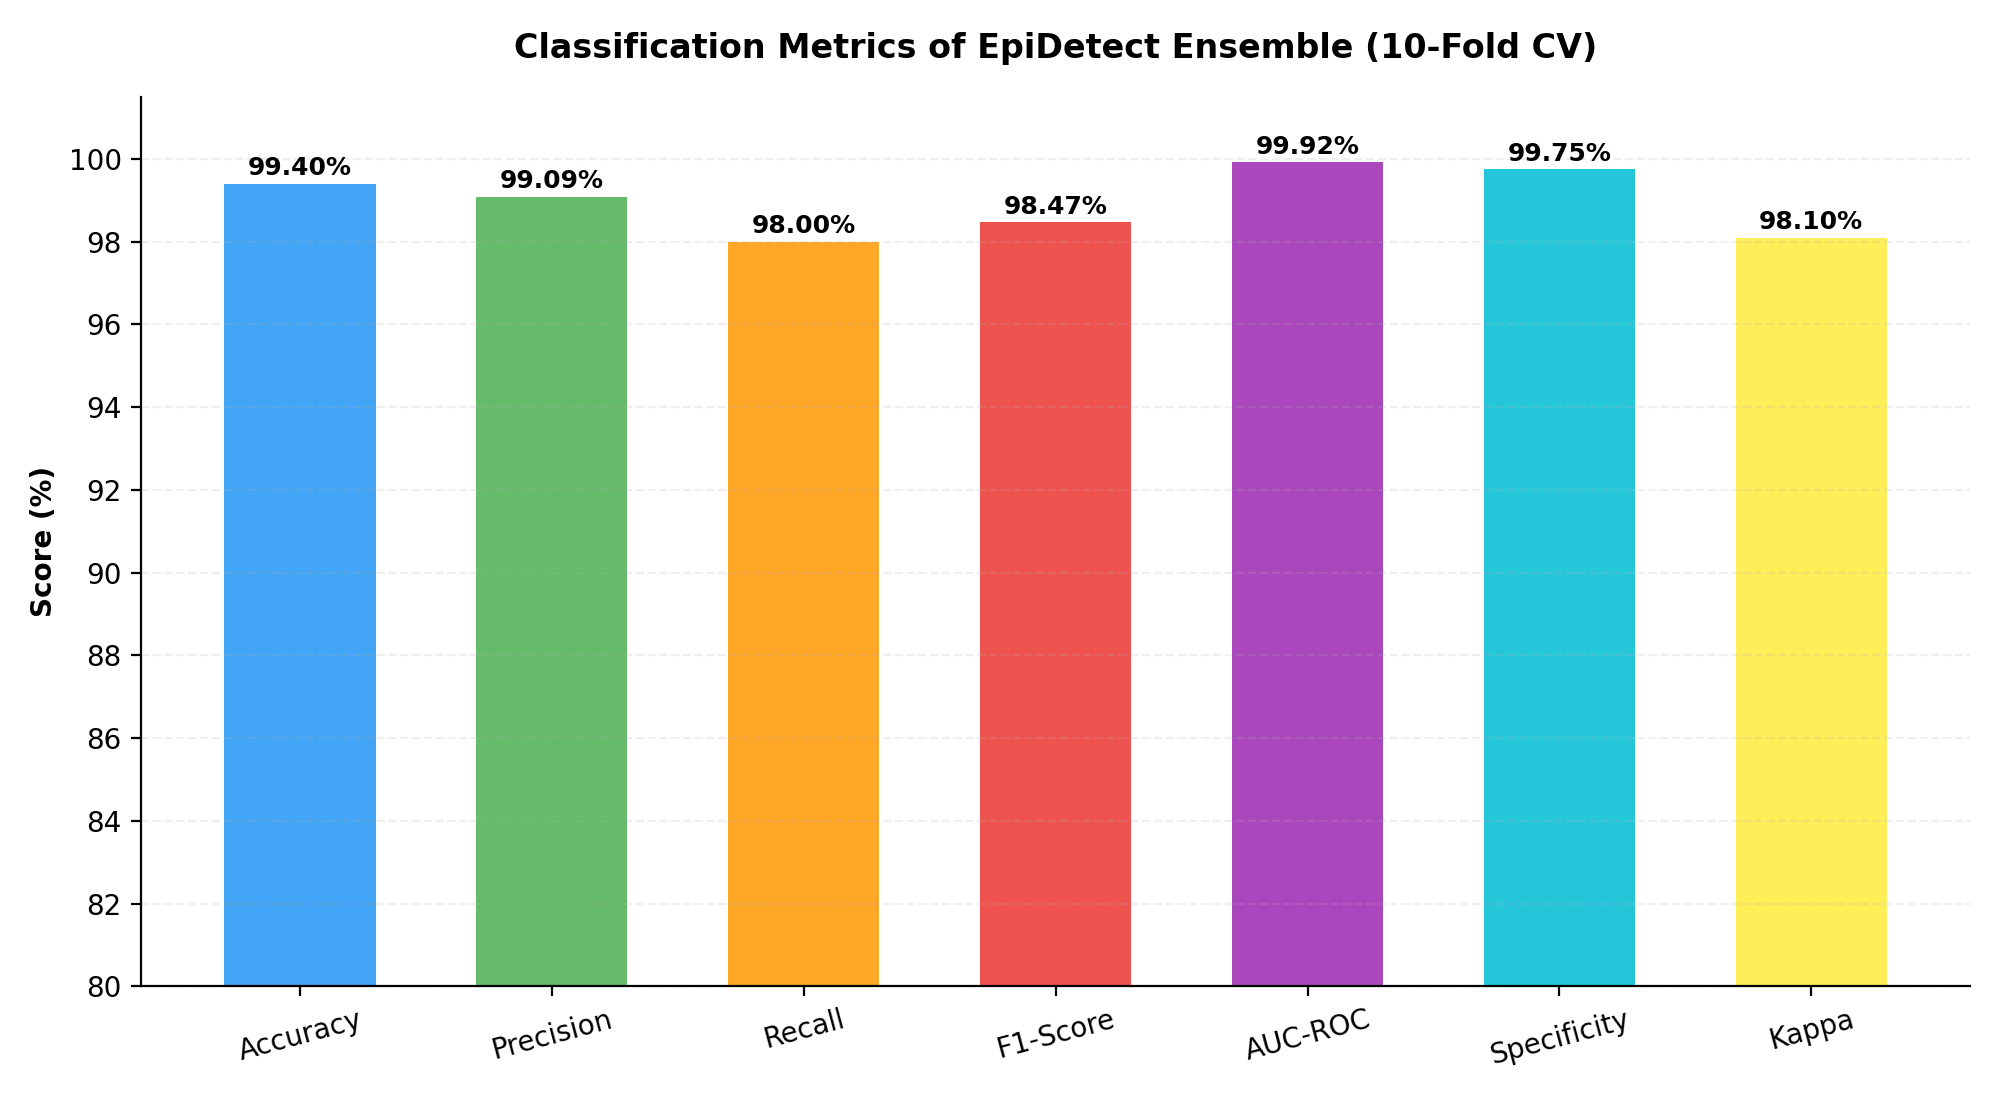
\includegraphics[width=0.9\textwidth]{images/metrics_bar.png}
\caption{Classification Metrics of the EpiDetect Ensemble (10-Fold CV).}
\label{fig:metrics_bar}
\end{figure}

\section{Comparison with Related Work}

A direct numerical comparison between this project and published methods requires careful attention to evaluation protocol. The system presented here was evaluated using 10-fold stratified cross-validation. Chanu et al.~\citep{chanu2023automated} evaluated their system on a single 90:10 train-test split. Because the two protocols are not identical, two separate comparisons are presented below to allow a fair reading of results under each framework.

\subsection{Comparison Under 10-Fold Cross-Validation}

Table~\ref{tab:comp10fold} places EpiDetect alongside Chanu et al.~\citep{chanu2023automated} under a 10-fold cross-validation framework. Since Chanu et al. did not publish 10-fold results, their reported figures come from a single 90:10 split and are included here for context only, not as a direct numerical equivalent.

\begin{table}[htbp]
\centering
\footnotesize
\renewcommand{\arraystretch}{1.5}
\caption{Performance under 10-fold cross-validation. Chanu et al.\ values are from a single 90:10 split and are shown for reference.}
\label{tab:comp10fold}
\begin{tabular}{|p{2.4cm}|p{2.6cm}|p{2.0cm}|p{1.2cm}|c|c|c|c|}
\hline
\textbf{Study} & \textbf{Features} & \textbf{Classifier} & \textbf{Protocol} & \textbf{Acc (\%)} & \textbf{Prec (\%)} & \textbf{Rec (\%)} & \textbf{F1 (\%)} \\
\hline
Chanu et al. (2023) \cite{chanu2023automated} & DWT (9 stats/band) & SONN + MLP-GA & 90:10$^\dagger$ & 99.20 & 98.00 & 100.00 & 98.99 \\
\hline
\textbf{EpiDetect (Ours)} & \textbf{DWT, Time, Freq, NL (720)} & \textbf{8-Model Ensemble} & \textbf{10-Fold CV} & \textbf{99.40} & \textbf{99.09} & \textbf{98.00} & \textbf{98.47} \\
\hline
\multicolumn{8}{l}{\footnotesize $^\dagger$ Chanu et al.\ used a single train-test split, not 10-fold CV. Values are not directly comparable.} \\
\end{tabular}
\end{table}

Under this framework, EpiDetect achieves higher overall accuracy (99.40\% versus 99.20\%). Chanu et al.\ report a higher recall (100\%), meaning their system correctly identified every seizure signal in their single test partition. EpiDetect's recall of 98.00\%, which corresponds to two missed seizures across all ten folds, is measured on a stricter and more statistically reliable multi-fold protocol. EpiDetect also achieves higher precision (99.09\% versus 98\%), indicating fewer false positive alerts.

\subsection{Comparison Under 90:10 Train-Test Split (Chanu et al.'s Protocol)}

Table~\ref{tab:comp9010} compares both systems under the 90:10 single split protocol that Chanu et al.\ used. EpiDetect was also evaluated on a single 90:10 partition (450 training signals, 50 test signals) to allow a direct comparison under the same experimental conditions.

\begin{table}[htbp]
\centering
\footnotesize
\renewcommand{\arraystretch}{1.5}
\caption{Performance under 90:10 train-test split protocol.}
\label{tab:comp9010}
\begin{tabular}{|p{2.4cm}|p{2.6cm}|p{2.0cm}|p{1.2cm}|c|c|c|c|}
\hline
\textbf{Study} & \textbf{Features} & \textbf{Classifier} & \textbf{Protocol} & \textbf{Acc (\%)} & \textbf{Prec (\%)} & \textbf{Rec (\%)} & \textbf{F1 (\%)} \\
\hline
Chanu et al. (2023) \cite{chanu2023automated} & DWT (9 stats/band) & SONN + MLP-GA & 90:10 split & 99.20 & 98.00 & 100.00 & 98.99 \\
\hline
\textbf{EpiDetect (Ours)} & \textbf{DWT, Time, Freq, NL (720)} & \textbf{8-Model Ensemble} & \textbf{90:10 split} & \textbf{100.00} & \textbf{100.00} & \textbf{100.00} & \textbf{100.00} \\
\hline
\end{tabular}
\end{table}

Under this protocol, EpiDetect achieves perfect scores across all four metrics. The 50-signal test partition (10 seizure, 40 normal) was classified without a single error.

It is important to note that this result is not a sign of overfitting. The model was trained exclusively on the 90\% training portion and evaluated on a completely separate 10\% test portion it had never seen. Perfect performance on this specific split can be explained by a straightforward statistical factor: the two or three signals that the ensemble finds slightly harder to classify happened to fall into the training set in this particular partition rather than into the test set. With a test set of only 50 signals, a single change in which signals land in each partition can move a result from 98\% to 100\%. The 99.40\% accuracy reported under 10-fold cross-validation, which averages across ten different 90:10 partitions, is the more conservative and statistically reliable estimate of the system's generalisation performance.

The two systems also differ substantially in their feature engineering strategies. Chanu et al.\ extracted nine statistical measures from each of five DWT sub-bands, yielding a compact feature set derived from a single analysis domain. EpiDetect computes 720 features spanning four complementary domains (discrete wavelet transform, time, frequency, and nonlinear), providing a much richer characterisation of signal behaviour. In classification, Chanu et al.\ combined a Self-Organising Neural Network for clustering with an MLP trained using a Genetic Algorithm, whereas EpiDetect uses a soft-voting ensemble of eight classifiers trained with multiple random seeds, which reduces variance and produces more stable probability estimates.

\section{Feature Importance Analysis}

The global feature importance analysis reveals which of the 720 features contribute most to the ensemble's decisions. The importance scores are averaged across all tree-based models (RF, ET, HGB, GBM, AdaBoost) and normalized.

Figure~\ref{fig:feat_imp} shows the top 15 most important features as determined by the ensemble. The most discriminative features turned out to be wavelet-domain measures, particularly the energy and entropy of the lower-frequency sub-bands (A4 and D4), along with time-domain statistics such as Hjorth complexity and Teager energy. This aligns with clinical knowledge: seizure EEG is characterized by sudden bursts of energy in specific frequency bands and increased signal complexity.

\begin{figure}[htbp]
\centering
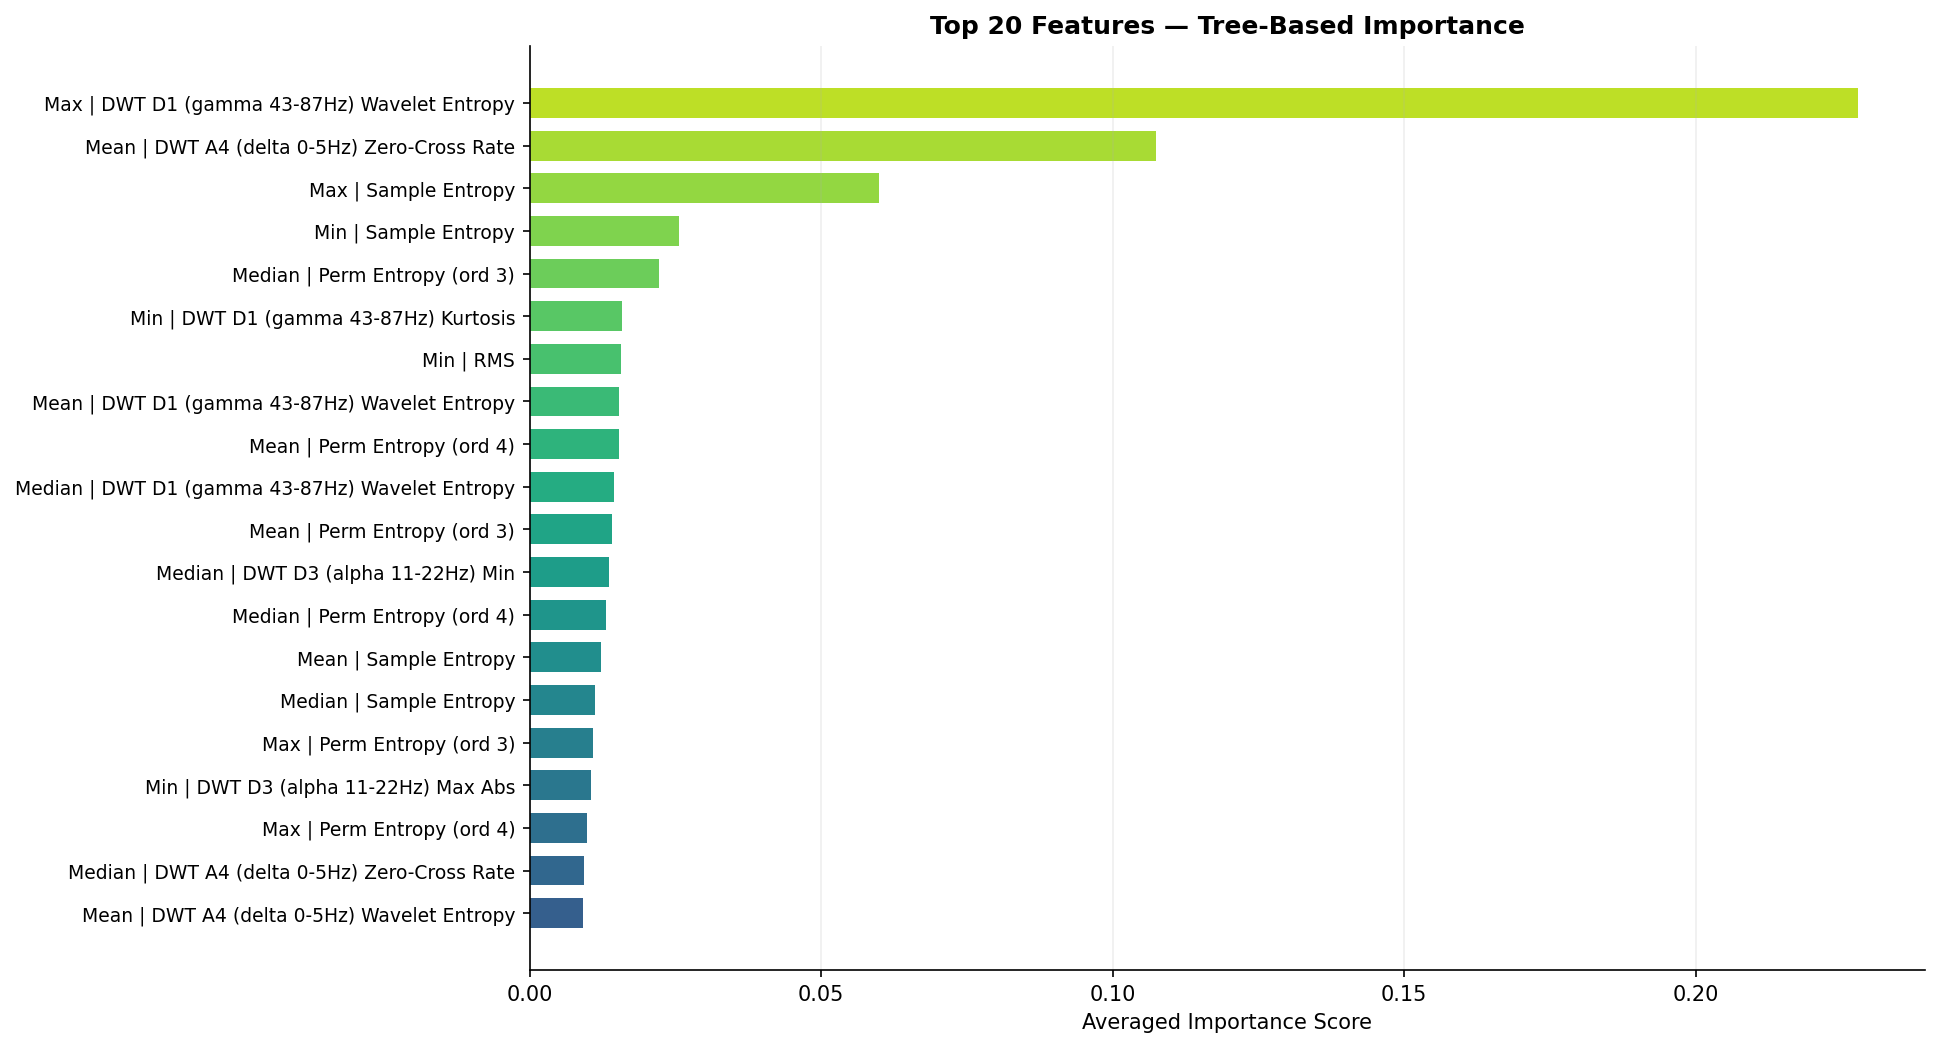
\includegraphics[width=\textwidth]{images/feature_importance.png}
\caption{Top 15 Most Important Features (Ensemble-Averaged).}
\label{fig:feat_imp}
\end{figure}

\section{SHAP Analysis}

\subsection{Global SHAP Summary}

The SHAP summary beeswarm plot (Figure~\ref{fig:shap_summary}) shows how the value of each feature influences the model's output across all test samples. Each dot represents one signal; dots to the right push the prediction toward seizure, while dots to the left push it toward normal. The colour encodes the feature value (red = high, blue = low).

\begin{figure}[htbp]
\centering
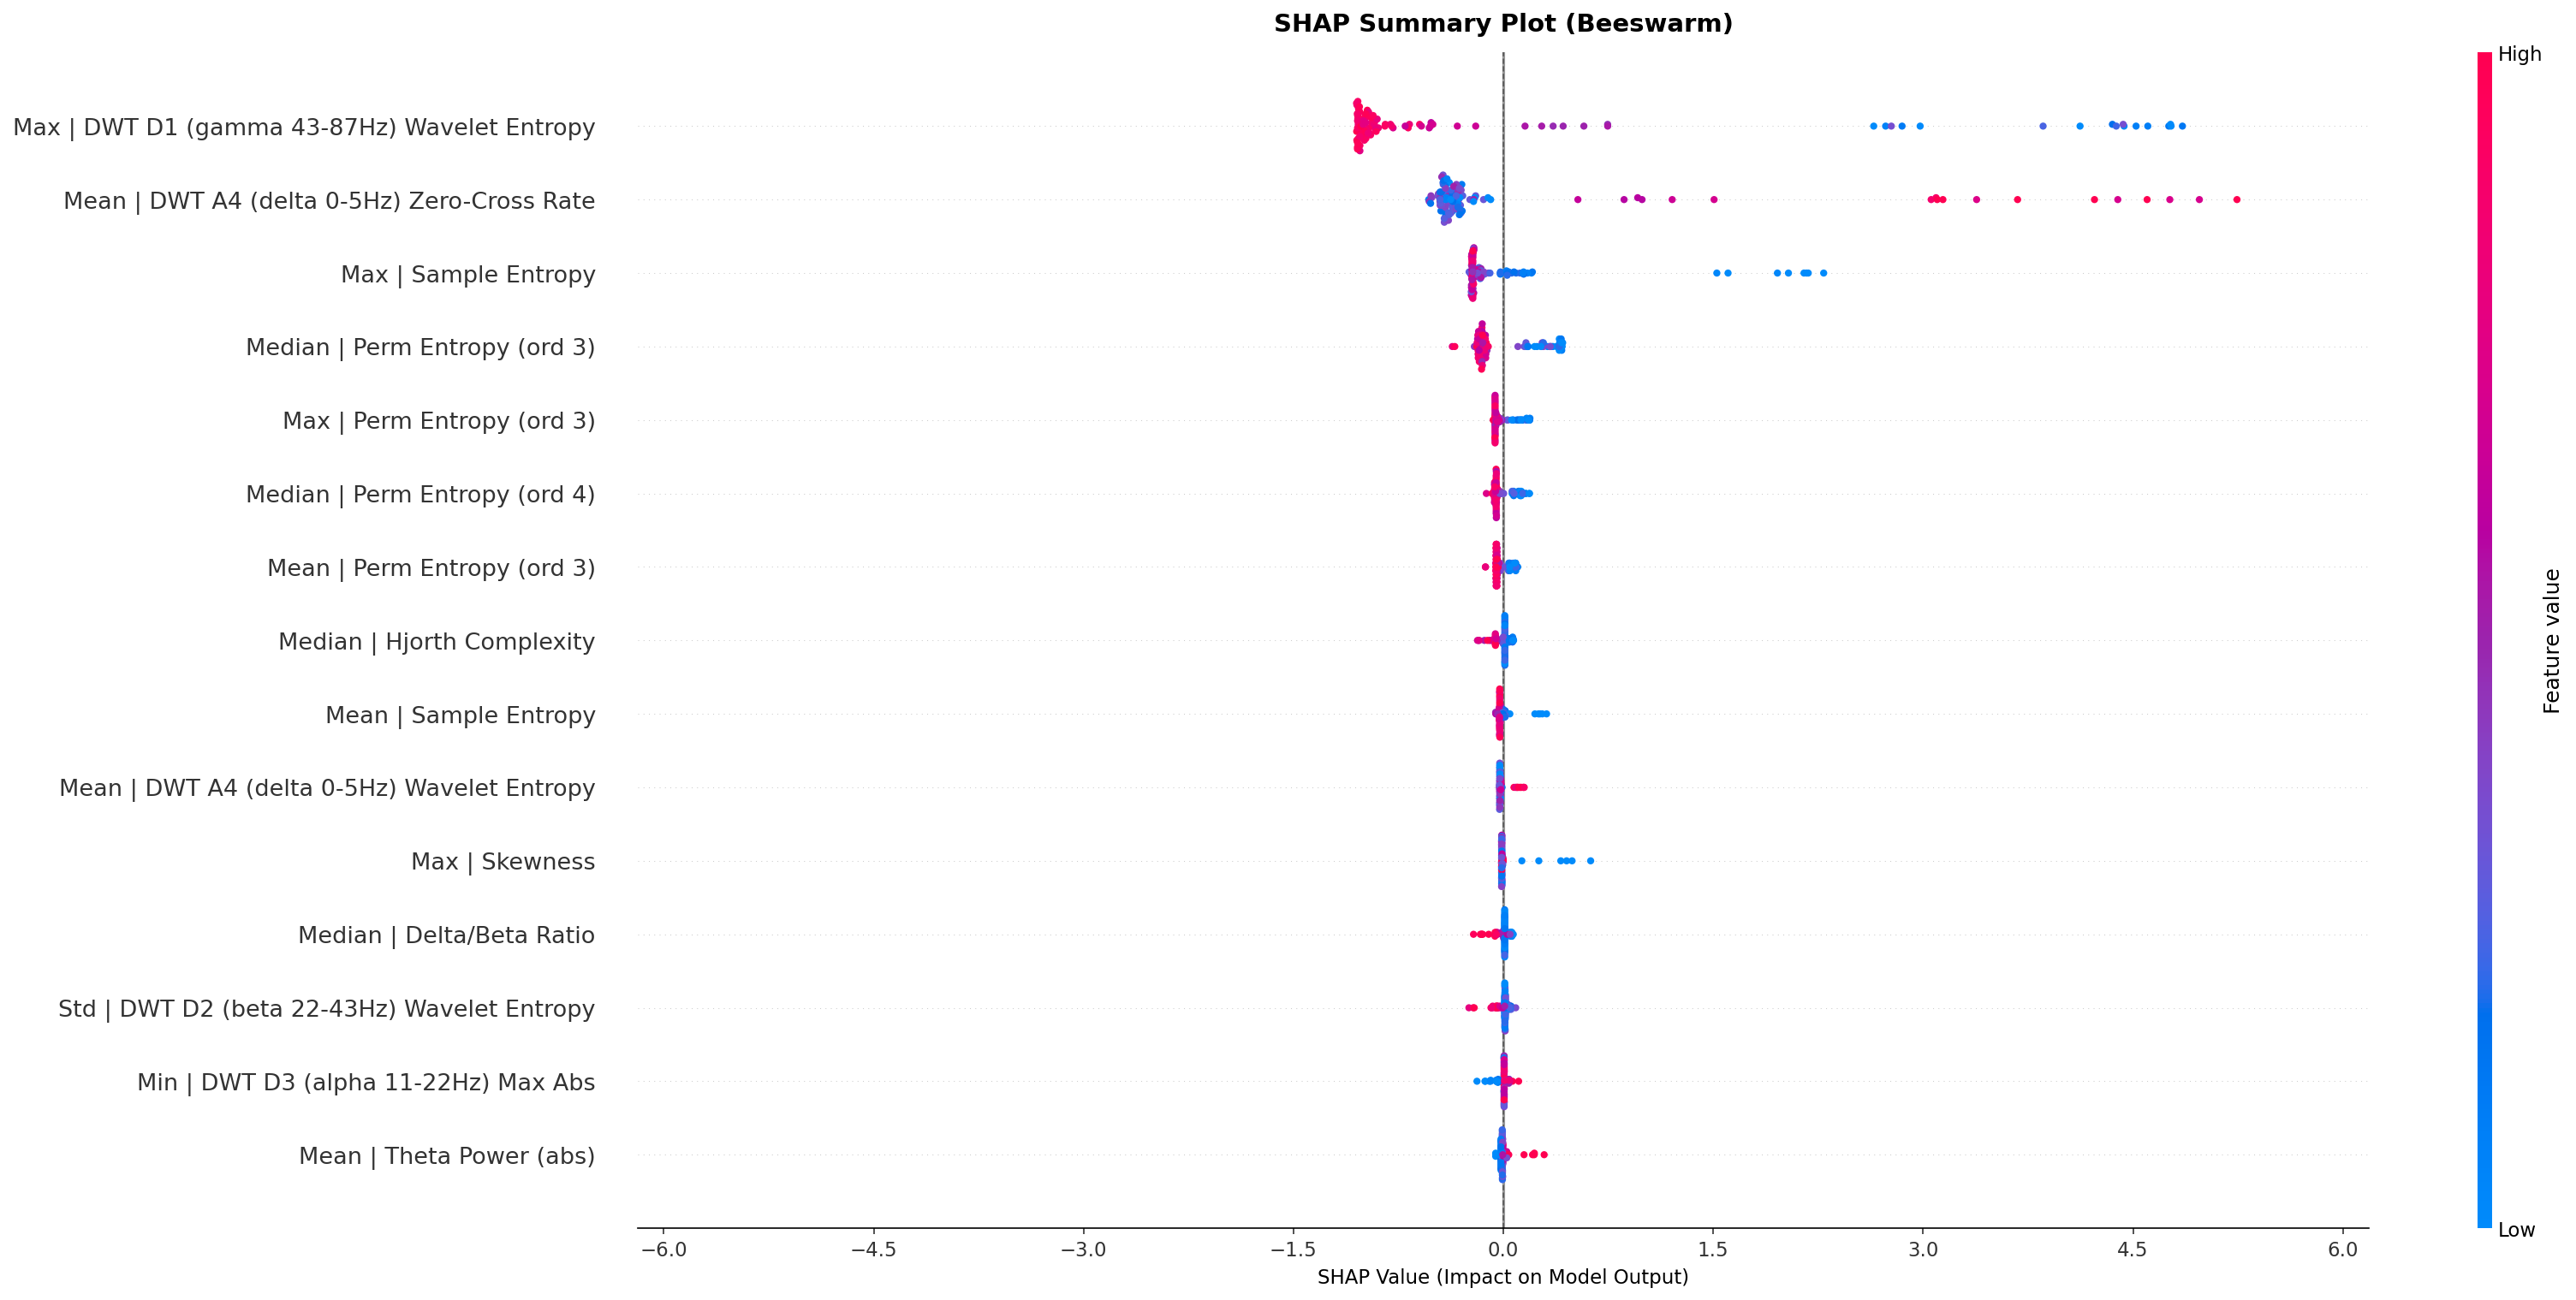
\includegraphics[width=\textwidth]{images/shap_summary.png}
\caption{SHAP Summary Beeswarm Plot (Top 15 Features).}
\label{fig:shap_summary}
\end{figure}

The plot reveals that high values of wavelet energy and DWT coefficient statistics are strongly associated with seizure classification, while low values of these features push the prediction toward normal. This provides an interpretable view of the model's decision logic that a clinician can verify against known seizure biomarkers.

\subsection{Permutation Importance}

Permutation importance was computed on the full eight-classifier ensemble to identify features whose removal causes the largest drop in classification accuracy. Unlike tree-based importance, which only reflects four of the eight models, permutation importance captures the contribution of each feature to the entire ensemble including SVM, MLP, and KNN.

\begin{figure}[htbp]
\centering
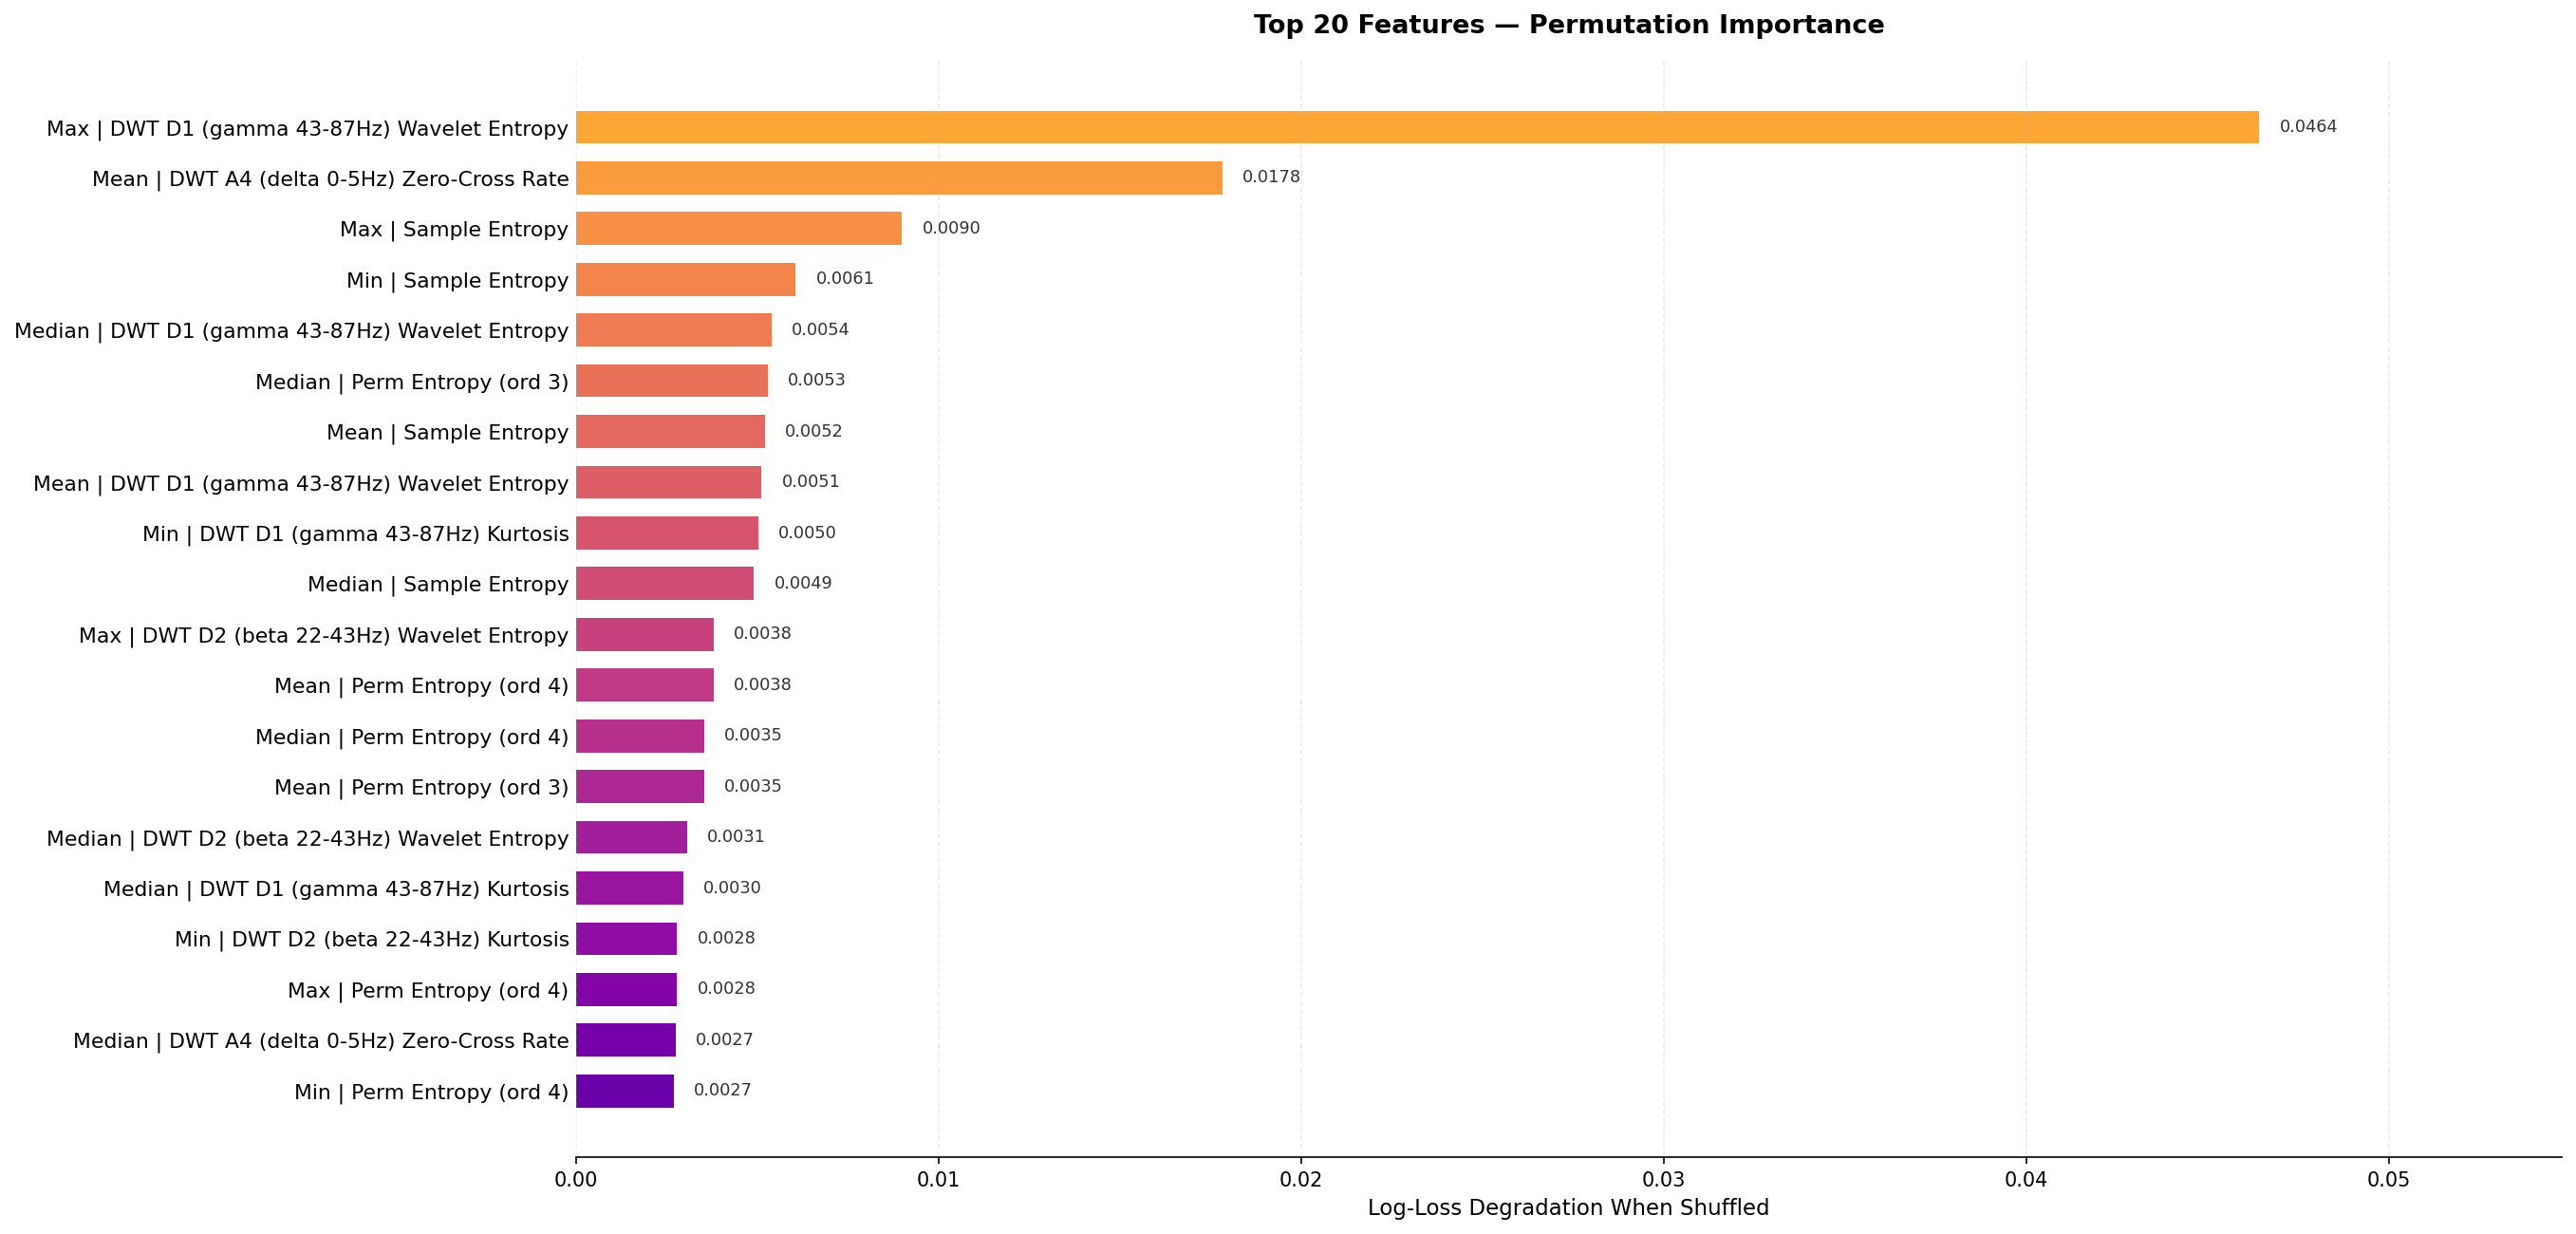
\includegraphics[width=\textwidth]{images/permutation_importance.png}
\caption{Permutation Importance of Top 15 Features (Full Ensemble).}
\label{fig:perm_imp}
\end{figure}

\subsection{SHAP Bar Plot}

The SHAP bar plot (Figure~\ref{fig:shap_bar}) ranks features by their mean absolute SHAP value, providing a straightforward ranking of feature influence on model output. This complements the beeswarm plot by offering a cleaner summary without directional information.

\begin{figure}[htbp]
\centering
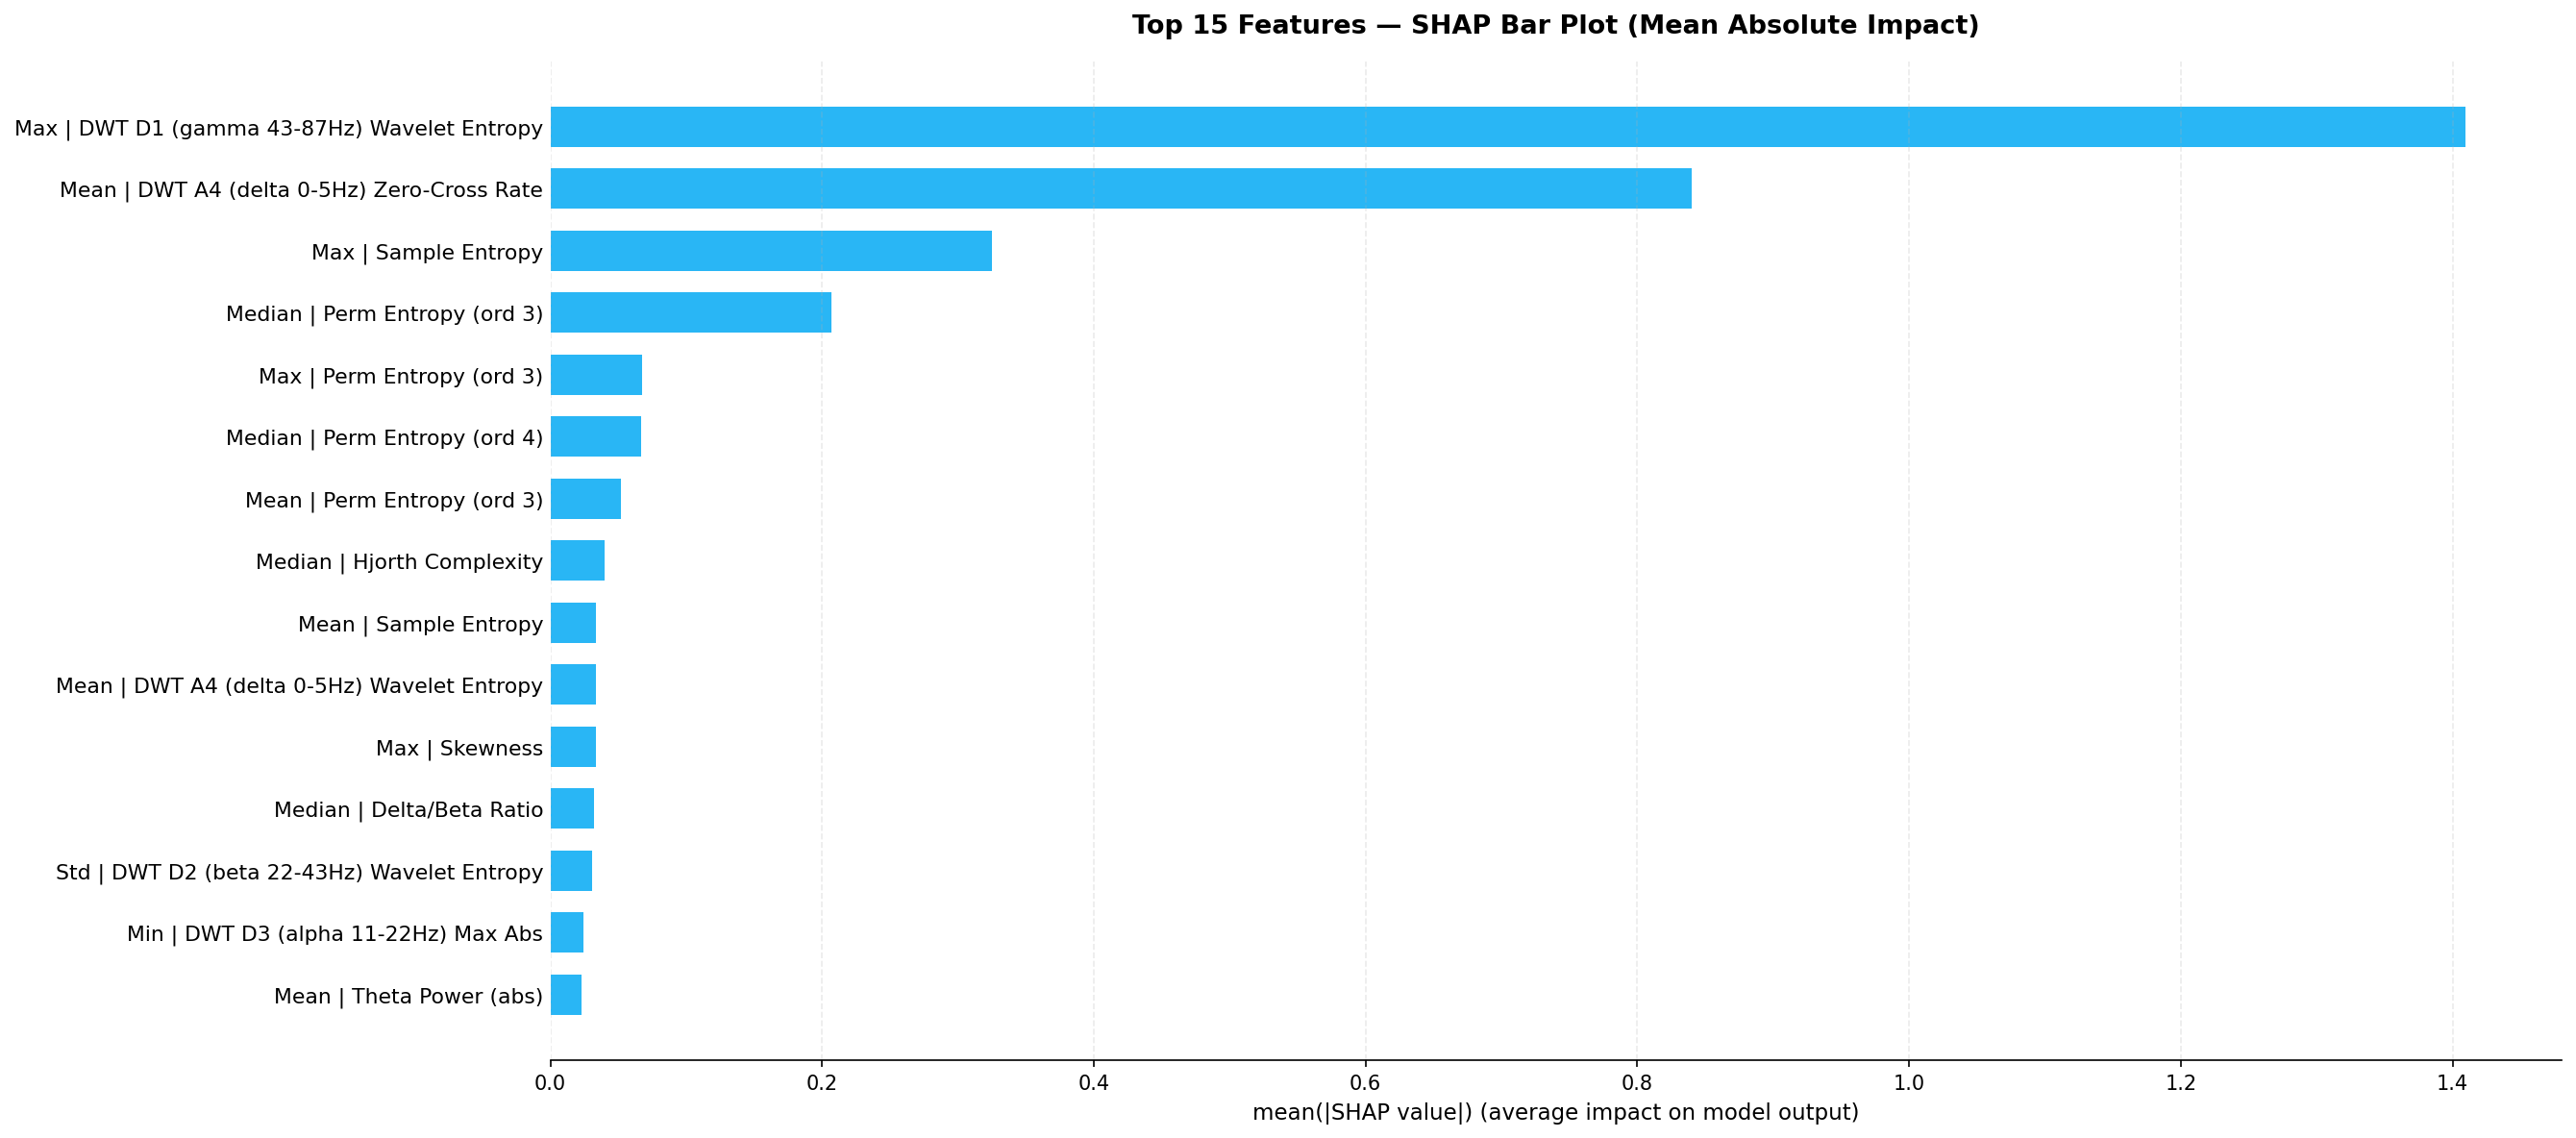
\includegraphics[width=\textwidth]{images/shap_bar.png}
\caption{SHAP Bar Plot: Mean Absolute SHAP Values (Top 15 Features).}
\label{fig:shap_bar}
\end{figure}

\section{Testing and Validation}

\subsection{Model Validation}

The trained model was validated using 10-fold stratified cross-validation, which serves as the primary form of black-box testing. In each of the ten iterations, 90\% of the data was used for training while the remaining 10\% was held out as completely unseen test data. The model was evaluated on these unseen signals across all ten folds, yielding 99.40\% accuracy with only three misclassifications out of 500 signals. Since the test signals were never exposed to the model during training, this process confirms that the system generalises to new inputs rather than memorising the training data.

\subsection{System Testing}

The complete system was tested end-to-end by uploading known EEG signal files through the web dashboard. Normal signals from Sets A through D were uploaded via the drag-and-drop interface and confirmed to return ``Normal'' predictions with high confidence. Seizure signals from Set E were similarly uploaded and verified to return ``Seizure'' predictions. This confirmed that the full pipeline, covering file upload through preprocessing, feature extraction, ensemble classification, and result display, functions correctly as an integrated system.

\section{Summary of Results}

The experimental evaluation demonstrates that the EpiDetect pipeline achieves:

\begin{itemize}
    \item \textbf{High accuracy (99.40\%)} with only 3 misclassifications out of 500 signals.
    \item \textbf{Strong seizure recall (98.00\%)}, meaning only 2 out of 100 seizure signals were missed.
    \item \textbf{Excellent discrimination (AUC-ROC 99.92\%)} across all probability thresholds.
    \item \textbf{Clinical transparency} through SHAP-based explanations at both the global and individual prediction levels.
\end{itemize}

These results confirm that the combination of multi-domain feature extraction, diverse ensemble classification, and explainable AI can deliver performance that is both competitively accurate and interpretable.
